\documentclass[11pt]{article}
\usepackage{latexsym}
\usepackage{amsmath}
\usepackage{amssymb}
\usepackage{amsthm}
\usepackage{epsfig}
\usepackage[tight]{subfigure}

\usepackage{amsmath}

\DeclareMathOperator*{\minimize}{min}
\DeclareMathOperator*{\maximize}{max}

\usepackage{algorithm}
 %on linux you may need to run sudo apt-get install texlive-full to install algorithm.sys
\usepackage{algorithmic}

\usepackage{verbatim}

\newcommand{\handout}[5]{
  \noindent
  \begin{center}
  \framebox{
    \vbox{
      \hbox to 5.78in { {#1} \hfill #2 }
      \vspace{4mm}
      \hbox to 5.78in { {\Large \hfill #5  \hfill} }
      \vspace{2mm}
      \hbox to 5.78in { {\em #3 \hfill #4} }
    }
  }
  \end{center}
  \vspace*{4mm}
}

\newcommand{\lecture}[5]{\handout{#1}{#2}{#3}{#4}{#5}}
\newcommand{\collision}[0]{\mathrm{collision}}
\newcommand{\nocollision}[0]{\overline{\collision}}

\newcommand*{\QED}{\hfill\ensuremath{\square}}

\newtheorem{theorem}{Theorem}
\newtheorem{corollary}[theorem]{Corollary}
\newtheorem{lemma}[theorem]{Lemma}
\newtheorem{observation}[theorem]{Observation}
\newtheorem{proposition}[theorem]{Proposition}
\newtheorem{definition}[theorem]{Definition}
\newtheorem{claim}[theorem]{Claim}
\newtheorem{fact}[theorem]{Fact}
\newtheorem{assumption}[theorem]{Assumption}
\newtheorem{note}[theorem]{Note}

% 1-inch margins, from fullpage.sty by H.Partl, Version 2, Dec. 15, 1988.
\topmargin 0pt
\advance \topmargin by -\headheight
\advance \topmargin by -\headsep
\textheight 8.9in
\oddsidemargin 0pt
\evensidemargin \oddsidemargin
\marginparwidth 0.5in
\textwidth 6.5in

\parindent 0in
\parskip 1.5ex
%\renewcommand{\baselinestretch}{1.25}

\begin{document}

\lecture{Statistical Techniques in Robotics (16-831, S22)}{Lecture \#03
  (Wednesday, January 26)}{Lecturer: Kris Kitani}{Scribes: John Harrington, Russell Wong (Group 1)}{PWEA Analyses \& Regret}

\section{Review}



%This section serves as a review of the previous lecture and any other context required to frame the content of the current lecture. 

%You may format the scribes in any way you like, aside from changing font style, size and page format. Please use subsections and paragraphs to increase the readability of your notes.

%Length requirement 1-2 pages.
        
\subsection{Online Learning}

In the previous lecture, we had been introduced the concept of online learning. In an online learning scenario, at a given time step $t$ the learner will make a prediction $\hat{y}^{(t)}$ about its environment or nature, based on some update parameters $\theta$ and possibly informed by an input or observation $\boldsymbol{x}^{(t)}$. The learner is then made aware of the true answer $y^{(t)}$, and in retrospect experiences a loss defined by a loss function $\ell(\hat{y}^{(t)}, y^{(t)})$. The learner then repeats this cycle for successive time steps, and updates its parameters $\theta$ based on the mistakes it has made in previous iterations, to better inform its future predictions. The hope is that the learner will tend towards reducing or minimizing loss in the long run (more generally, the goal of online learning is to reduce regret, which was introduced during this lecture and is described in detail in Section \ref{section:regret}).

\subsection{Prediction with Expert Advice}

We had also discussed the general concept of \textbf{PWEA} (Prediction with Expert Advice) in the previous lecture. This applies to one class of online learning problems, in which the robot learner has access to insights from so-called ``experts", who formulate their own predictions and can be used to inform the learner's decisions \cite{hoi2018online}. PWEA is characterized by being \textbf{Exhaustive} (since the action space is finite and can be completely tested), \textbf{Instructive} (since we receive a fully observable loss, knowing if each expert was correct), and \textbf{One-shot} (since the data arrives as a stream and the action taken does not affect the next state). We explored one type of PWEA algorithm, the Greedy Algorithm, which is analyzed in further detail in Section \ref{section:greedy}. We were introduced to the terminology of the instance domain $\mathcal{X}$, target domain $\mathcal{Y}$, and hypothesis class $\mathcal{H}$. The instance domain $\mathcal{X}$ is the set of all possible inputs or observations $\{x\in\mathcal{X}\}$. The target domain is the set of all possible outcomes or answers $\{y\in\mathcal{Y}\}$. The hypothesis class $\mathcal{H}$ is the set of functions that map inputs to outcomes, also known as the set of hypotheses $\{h:\mathcal{X}\rightarrow\mathcal{Y}\}$. 

\subsection{Realizability}

Finally, in the previous lecture we were introduced to \textbf{realizability}. Realizability represents an assumption in our online learning, that a perfect expert does exist within our set of hypotheses, and therefore can be found. The perfect hypothesis is denoted $h^\star\in\mathcal{H}$.

\section{Consistent Algorithm Mistake Bound}\label{section:mistake_bound}



When analyzing performance of an online learner, where its predictions can either yield correct or incorrect, one valuable metric is the number of mistakes an algorithm can make. In a PWEA problem, mistakes are made while the learner tests different hypotheses, in pursuit of finding the perfect expert (assuming realizability). Ideally, the learning algorithm would require fewer mistakes to be made in order to find the perfect expert; therefore, by analytically determining an upper bound for the number of mistakes made, expected performance can be evaluated.

Throughout the notes, the bound derivation will follow this pattern:
\begin{enumerate}
    \item Define a \textbf{Potential Function}, representing the size of the version space
    \item Determine the \textbf{Upper Bound} of the potential function after increment (another mistake)
    \item Determine the \textbf{Lower Bound} of the potential function (often comparably trivial but important for later steps) 
    \item \textbf{Combine Bounds} determined in Steps 2 and 3
    \item \textbf{Determine Performance Bounds} of the algorithm through algebraic manipulation or approximation methods 
\end{enumerate}

The significance of finding theoretical bounds on these algorithms is that it imposes a mathematical guarantee on the performance bounds. This means we can develop a robotic system (or other application) that can learn with some level of expectation. 


\section{Greedy Algorithm}\label{section:greedy}

\subsection{Overview}

The Greedy Algorithm was described during the last lecture, but will act as a simple example to work through the performance bound derivation. 

Let $\boldsymbol{V}^{(t)}$ be the version space at time step $t$, $\mathcal{H}$ be the hypothesis class, $T$ be the maximum time step (assumed to be infinity), $\boldsymbol{x}^{(t)}$ be the input or observation at time step $t$, and $y^{(t)}$ be the true outcome at time step $t$.

The Greedy Algorithm is presented in Algorithm \ref{algo:greedy}:

\begin{algorithm}[H]
\caption{Greedy Algorithm}
\label{algo:greedy}
\begin{algorithmic}[1]
\STATE $\boldsymbol{V}^{(1)} = \mathcal{H}$  \hfill $\triangleright$ Version space initialization
\FOR{$t=1,\;\dots,\;T$}
\STATE \textsc{Receive} ($\boldsymbol{x}^{(t)}$) \hfill $\triangleright$ Receive expert predictions
\STATE $h = \textsc{FirstElem} (\boldsymbol{V}^{(t)})$ \hfill $\triangleright$ Greedy selection of first element in the version space
\STATE $\hat{y}^{(t)} = h(\boldsymbol{x}^{(t)})$ \hfill $\triangleright$ Make prediction based on selection
\STATE \textsc{Receive} ($y^{(t)}$) \hfill $\triangleright$ Receive true outcome
\STATE $\boldsymbol{V}^{(t+1)} = \big\{ h \in \boldsymbol{V}^{(t)} : h(\boldsymbol{x}^{(t)}) = y^{(t)} \big\} $ \hfill $\triangleright$ Keep only `consistent' hypotheses
\ENDFOR
\end{algorithmic}
\end{algorithm}

Line 4, the update step of the algorithm, simply picks the first candidate based on the existing ordering of hypothesis in the version space, and no other information (hence the greedy name). Then in Line 7, all of the hypotheses are tested against the true outcome, and the ones that made a mistake are discarded.

\subsection{Bounds Derivation}

\theorem{Let $M$ be the number of mistakes made by a learner using the Greedy Algorithm, and let $\mathcal{H}$ be the hypothesis class. The number of mistakes $M$ is bounded by:

$$M \le |\mathcal{H}|-1$$
}

\proof{
We execute the derivation steps outlined in Section \ref{section:mistake_bound}.}

\textbf{Potential Function:
}    
The potential function $|\boldsymbol{V}(t)|$ represents the number of valid hypotheses at time $t$.

\textbf{Upper Bound:}

We will consider what will happen to the potential function after one mistake is made by our algorithm. In the worst case, it is possible that our greedy choice picked the only incorrect hypothesis, meaning that our potential function would only shrink by one. 

$$|\boldsymbol{V}^{(t+1)}| \leq |\boldsymbol{V}^{(t)}| - 1$$

We know that the potential function will shrink after a mistake (since at least one hypothesis has been proven invalid by definition). Extrapolating this inequality, if we begin with the initial hypothesis class $|\mathcal{H}|$, and make mistakes, this would mean that the version space would shrink by at least $M$ after $M$ mistakes by induction, leading to the following upper bound:

\begin{equation}
\centering
|\boldsymbol{V}^{(t)}| \leq |\mathcal{H}| - M
\label{eq:greedy-upper-bound}    
\end{equation}

\textbf{Lower Bound: 
}
There will always be at least one expert in the version space, because we assume realizability. Hence, we know that the version space is lower bound by $1$:

\begin{equation}
\centering
|\boldsymbol{V}^{(t)}| \ge 1
\label{eq:greedy-lower-bound}
\end{equation}

\textbf{Combine Bounds:
}
Combining the Equations (\ref{eq:greedy-upper-bound}) and (\ref{eq:greedy-lower-bound}), the intermediate potential function can be removed as follows:

$$1 \leq |\boldsymbol{V}^{(t)}| \leq |\mathcal{H}| - M$$

$$1 \leq |\mathcal{H}| - M$$

\textbf{Determine Performance Bounds:
}

We can rearrange this equality to determine a performance bound on the number of mistakes $M$:

$$M \leq |\mathcal{H}| - 1$$


This gives us a performance guarantee linear in the size of the hypothesis class, and proves that the learner will make at most $ |\mathcal{H}| - 1$ mistakes in order to find the perfect hypothesis \cite{shalev-shwartz}. By improving our prediction heuristic we can do better, as can be seen in the Halving Algorithm described in Section \ref{section:halving}.

\section{Halving (Majority) Algorithm}\label{section:halving}

\subsection{Overview}

The Halving Algorithm follows similarly to the Greedy Algorithm, but with one key difference. Instead of naively picking the first element in our current version space, we determine what is called the \textbf{Majority Consensus} of the current version space. This simply means predicting using the majority vote of the consistent hypotheses \cite{shalev-shwartz}. The Halving Algorithm is depicted in Algorithm \ref{algo:halving}.

\begin{algorithm}[H]
\caption{Halving (Majority) Algorithm}
\label{algo:halving}
\begin{algorithmic}[1]
\STATE $\boldsymbol{V}^{(1)} = \mathcal{H}$  \hfill $\triangleright$ Version space initialization
\FOR{$t=1,\;\dots,\;T$}
\STATE \textsc{Receive} ($\boldsymbol{x}^{(t)}$) \hfill $\triangleright$ Receive expert predictions
\STATE $\hat{y}^{(t)} = \textsc{MajorityConsensus} (\boldsymbol{V}^{(t)})$ \hfill $\triangleright$ Choose prediction from majority choice
\STATE \textsc{Receive} ($y^{(t)}$) \hfill $\triangleright$ Receive true outcome
\STATE $\boldsymbol{V}^{(t+1)} = \big\{ h \in \boldsymbol{V}^{(t)} : h(\boldsymbol{x}^{(t)}) = y^{(t)} \big\} $ \hfill $\triangleright$ Keep only `consistent' hypotheses
\ENDFOR
\end{algorithmic}
\end{algorithm}

\subsection{Bounds Derivation}

\theorem{Let $M$ be the number of mistakes made by a learner using the Halving (Majority) Algorithm, and let $\mathcal{H}$ be the hypothesis class. The number of mistakes, $M$, is bounded by:

$$M \leq \log_2{|\mathcal{H}|}$$
}

\proof{
We execute the derivation steps outlined in Section \ref{section:mistake_bound}.}

\textbf{Potential Function:
}    
The potential function $|\boldsymbol{V}^{(t)}|$ represents the number of valid hypotheses at time $t$.

\textbf{Upper Bound:
}
We will consider what will happen to the potential function after one mistake is made by our algorithm. In all cases, the learner is matching its prediction with what is predicted by the majority (with some implementation-specific tie-breaking mechanism, such as a fixed ordering of which hypotheses take precedent over others in a tie). Therefore, when a mistake is made, it means that the majority is wrong, and at least half of the version space is invalidated. Thus, we have the following inductive relation:

$$|\boldsymbol{V}^{(t+1)}| \leq \frac{1}{2} |\boldsymbol{V}^{(t)}| $$

Similarly to the Greedy Algorithm, using a base case of $|\boldsymbol{V}^{(1)}| = |\mathcal{H}|$, we can extend this inequality for $M$ mistakes through induction. This leads to the following representation of the potential function with respect to the size of the original version space:

\begin{equation}
\centering
|\boldsymbol{V}^{(t)}| \leq  2^{-M}|\mathcal{H}|
\label{eq:halving-upper-bound}
\end{equation}

\textbf{Lower Bound:} 

Similar to the Greedy Algorithm, due to the realizability assumption, we know that the version space is lower bound by one.

\begin{equation}
\centering
|\boldsymbol{V}^{(t)}| \ge 1
\label{eq:halving-lower-bound}
\end{equation}

\textbf{Combine Bounds:}

Combining Equations (\ref{eq:halving-upper-bound}) and (\ref{eq:halving-lower-bound}) leads to the following inequality:

$$1 \leq |\boldsymbol{V}^{(t)}| \leq  2^{-M}|\mathcal{H}|$$

$$1 \leq 2^{-M}|\mathcal{H}|$$

\textbf{Determine Performance Bounds:}

Through some algebraic manipulation (taking the logarithm to the base 2 on both sides and isolating $M$), a mistake bound can be established:



$$\log_2{1} \leq \log_2\left({2^{-M}|\mathcal{H}|}\right)$$

$$0 \leq \log_2\left({2^{-M}|\mathcal{H}|}\right)$$

$$0 \leq -M + \log_2{|\mathcal{H}|}$$

$$M \leq \log_2{|\mathcal{H}|}$$

This performance bound is drastically improved from the Greedy Algorithm. Instead of simply guaranteeing that each mistake will remove at least one hypothesis from the version space, we can ensure that the entire version space will half each time at minimum (hence the algorithm name)! However, as noted above, all of the Prediction with Expert Advice algorithms discussed thus far apply only in the \textbf{exhaustive} case with finite experts and features.

\section{Randomized Greedy Algorithm}

\subsection{Overview}

The Randomized Greedy Algorithm, presented in Algorithm \ref{algo:random-greedy}, is another learning algorithm with one small change from the Greedy Algorithm. The key difference is that instead of taking the first hypothesis of the current version space, a random hypothesis is sampled from the current version space according to a uniform distribution. The rest of the algorithm follows identically to the original Greedy Algorithm described in Algorithm \ref{algo:greedy}.

\begin{algorithm}[H]
\caption{Randomized Greedy Algorithm}
\label{algo:random-greedy}
\begin{algorithmic}[1]
\STATE $\boldsymbol{V}^{(1)} = \mathcal{H}$  \hfill $\triangleright$ Version space initialization
\FOR{$t=1,\;\dots,\;T$}
\STATE \textsc{Receive} ($\boldsymbol{x}^{(t)}$) \hfill $\triangleright$ Receive expert predictions
\STATE $h \sim \textsc{Uniform} (\boldsymbol{V}^{(t)})$ \hfill $\triangleright$ Random Sample from Uniform Distribution
\STATE $\hat{y}^{(t)} = h(\boldsymbol{x}^{(t)})$ \hfill $\triangleright$ Choose prediction from chosen sample
\STATE \textsc{Receive} ($y^{(t)}$) \hfill $\triangleright$ Receive true outcome
\STATE $\boldsymbol{V}^{(t+1)} = \big\{ h \in \boldsymbol{V}^{(t)} : h(\boldsymbol{x}^{(t)}) = y^{(t)} \big\} $ \hfill $\triangleright$ Keep only `consistent' hypotheses
\ENDFOR
\end{algorithmic}
\end{algorithm}

\subsection{Bounds Derivation}

\theorem{Let $M^{(T)}$ be the expectation of total number of mistakes made by a learner up to time step $T$ using the Randomized Greedy Algorithm, and let $\mathcal{H}$ be the hypothesis class. The expectation of the number of mistakes, $M^{(T)}$, is bounded by:

$$M^{(T)} \leq \ln{|\mathcal{H}|}$$
}

\proof{
We execute the derivation steps outlined in Section \ref{section:mistake_bound}.}

\textbf{Potential Function:}
    
The potential function $|\boldsymbol{V}(t)|$ represents the number of valid hypotheses at time $t$.

\textbf{Upper Bound:}

At every time step, there exists some ratio of remaining experts, representing the probability that the remaining experts correctly predict the current trial. This number is both unknown and time varying, due to the probabilistic nature of the uniform sampling of hypotheses at each time step. We will define $\alpha(t)$ as the ratio of remaining experts after time step $t$:

\begin{equation}
\centering
|\boldsymbol{V}^{(t+1)}| = \alpha^{(t)} \cdot |\boldsymbol{V}^{(t)}|
\label{eq:alpha}
\end{equation}

As seen before, this incremental step can be extended via induction to determine the number of elements in the version space after $T$ trials. 

\begin{equation}
\centering
|\boldsymbol{V}^{(T+1)}| = |\mathcal{H}| \cdot \prod_{t=1}^T \alpha^{(t)}
\label{eq:random-greedy-product}
\end{equation}

Note: The above notation represents the product notation, where: $\prod_{t=1}^T \alpha^{(t)} = \alpha^{(1)} \cdot \alpha^{(2)} \dots \alpha^{(T-1)} \cdot \alpha^{(T)}$.

In order to transform this product into a summation, we can use the following inequality. For some $b$:

$$ b \leq e^{-(1-b)} $$ 

Substituting $b$ with $\alpha(t)$, we can use this relation in conjunction with Equation (\ref{eq:random-greedy-product}). Due to the ordering of the inequalities, this means that the $\alpha(t)$ term can be directly replaced as seen below:

$$ |\mathcal{H}| \cdot \prod_{t=1}^T \alpha^{(t)} \leq |\mathcal{H}| \cdot \prod_{t=1}^T e^{-(1-\alpha^{(t)})}$$

Using exponent rules, the product can then be converted into a summation in terms of $\alpha(t)$:

$$|\mathcal{H}| \cdot \prod_{t=1}^T e^{-(1-\alpha^{(t)})} = |\mathcal{H}| \cdot e^{- \sum_{t=1}^T (1-\alpha^{(t)})} $$


This results in the following expression for the version space upper bound:

\begin{equation}
\centering
|\boldsymbol{V}^{(T+1)}| \leq |\mathcal{H}| \cdot e^{- \sum_{t=1}^T (1-\alpha^{(t)})}
\label{eq:random-greedy-upper-bound}
\end{equation}

This inequality represents the upper bound on the version space at each time interval, as dependent on $\alpha(t)$. Recall from Equation (\ref{eq:alpha}) that we define $\alpha(t)$ as: 

$$|\boldsymbol{V}^{(t+1)}| = \alpha^{(t)} \cdot |\boldsymbol{V}^{(t)}|$$
$$ \alpha^{(t)} = \frac{|\boldsymbol{V}^{(t+1)}|}{|\boldsymbol{V}^{(t)}|} $$
In other words, $\alpha(t)$ represents the ratio of consistent hypotheses at a specific time step $t$, giving the proportion of hypotheses which will not make a mistake at that time step. Consequently, it also represents the probability of the algorithm not making a mistake at time $t$, meaning $1-\alpha(t)$ would represent the probability of the learner making a mistake at time $t$. We can express this in terms of \textbf{probability of making a mistake} at time step $t$, $p(\hat{y}^{(t)} \neq y^{(t)})$, which can be equivalently thought of as the \textbf{expectation that the learner will make a mistake} at time step $t$, over the distribution of possible predictions $p(\hat{y})$.

$$1 - \alpha(t) = p(\hat{y}^{(t)} \neq y^t) = \mathbb{E}_{p(\hat{y})} \bigg[ \textbf{1} [\hat{y}^{(t)} \neq y^t] \bigg] $$

Here, expectation is denoted with the symbol $\mathbb{E}$. Using this concept, we can calculate the \textbf{expectation of the total number of mistakes} the algorithm will make over a set number of time steps through a summation. The expectation of total mistakes made up to time step $T$ is denoted $M^{(T)}$, and is given by:

\begin{equation}
\centering    
M^{(T)} =  \sum_{t=1}^T\mathbb{E}_{p(\hat{y})} \bigg[ \textbf{1}  [\hat{y}^{(t)} \neq y^t] \bigg] = \sum_{t=1}^T (1 - \alpha(t)) \label{eq:total-mistakes-expectation}
\end{equation}

Interestingly, this summation also appears in our version space upper bound from Equation (\ref{eq:random-greedy-upper-bound})! By substituting Equation (\ref{eq:total-mistakes-expectation}) into Equation (\ref{eq:random-greedy-upper-bound}), we achieve the following expression for an upper bound, in terms of the expectation of total mistakes $M^{(T)}$:

\begin{equation}
\centering
|\boldsymbol{V}^{(T+1)}| \leq |\mathcal{H}| \cdot e^{- M^{(T)}}
\label{eq:random-greedy-upper-bound-2}
\end{equation}

\textbf{Lower Bound:} 

Once again, due to the realizability assumption, we recognize that the version space is lower bound by one.

\begin{equation}
\centering
|\boldsymbol{V}^{(T+1)}| \ge 1
\label{eq:random-greedy-lower-bound}
\end{equation}

\textbf{Combine Bounds:}

Combining Equations (\ref{eq:random-greedy-upper-bound-2}) and (\ref{eq:random-greedy-lower-bound}) yields the following:

$$1 \leq |\boldsymbol{V}^{(t+1)}| \leq |\mathcal{H}| \cdot e^{-M^{(T)}}$$

$$1 \leq \mathcal{H} \cdot e^{-M^{(T)}}$$

\textbf{Determine Performance Bounds}:

Taking the natural logarithm and rearranging terms:

$$0 \leq \ln{|\mathcal{H}|} - M^{(T)}$$

$$ M^{(T)} \leq \ln{|\mathcal{H}|}$$

Compared to the halving algorithm, which was upper bound by $\log_2 |\mathcal{H}|$, this is a slightly better bound. Figure \ref{fig:mistake-bound-comparison} illustrates the asymptotic behavior of mistake bounds for each of the algorithms explored thus far. However, it is important to note that in the case of the halving algorithm, the bound was a worst case bound, compared to the expected mistake bound.

\begin{figure}[H]
    \centering
    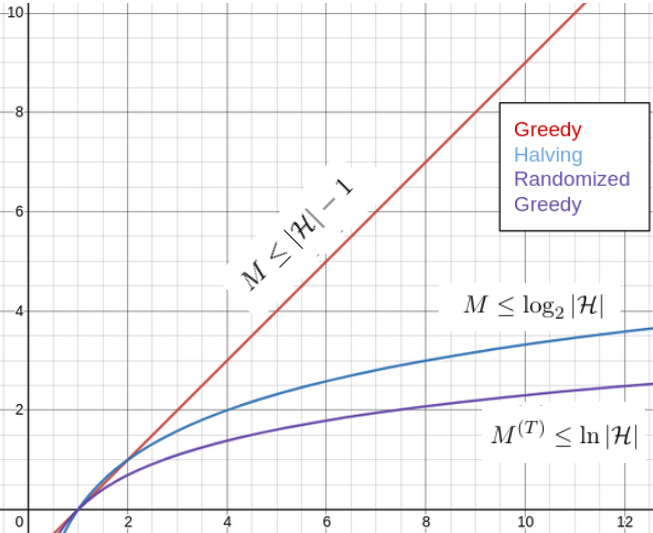
\includegraphics[width=10cm]{function_comparison.png}
    \caption{Comparison of  Mistake Bounds from Different PWEA Algorithms}
    \label{fig:mistake-bound-comparison}
\end{figure}

\section{Regret}\label{section:regret}

\subsection{Motivation}

In the aforementioned examples, it is assumed that there exists a perfect hypothesis $h^\star\in\mathcal{H}$ such that $h^\star:\mathcal{X}\rightarrow\mathcal{Y}$. The existence of $h^\star$ in the hypothesis class is referred to as \textbf{realizability} \cite{shalev-shwartz}. Under this assumption, the lower bound of the size of the version space is given by:

$$ 1 \leq |\boldsymbol{V}^{(t)}|$$

This makes it possible to place bounds on the maximum number of mistakes that can be made, as a function of the size of the hypothesis class.

However, this approach falls apart when realizability no longer holds. Without the existence of a perfect hypothesis in the hypothesis class, it is possible for the version space to eventually become empty, as all experts are now capable of making a mistake. This necessitates an alternate method for measuring performance; one that does not rely strictly on mistake bounds. Rather than evaluating performance against a perfect hypothesis, performance can be evaluated in relation to the best-performing hypothesis in $\mathcal{H}$. This idea sets the foundation for the concept of \textbf{regret}.

\subsection{Regret Bounds and Definition of Regret}

A \textbf{regret bound} is a general concept used to evaluate the performance of a learning algorithm. \textbf{Mistake bounds} that have been established previously are a special type of regret bounds.

The regret $R$ of a learner at time step $T$ in relation to a particular hypothesis $h\in\mathcal{H}$ is defined by:

$$ R^{(T)}(h) = \sum_{t=1}^T{\ell(\hat{y}^{(t)},y^{(t)})} - \sum_{t=1}^T{\ell(h(\boldsymbol{x}^{(t)}),y^{(t)})} $$
 
Where $\hat{y}^{(t)}$ is the prediction made by the learner at time $t$, $\boldsymbol{x}^{(t)}$ is the input or observation at time $t$, and $h(\boldsymbol{x}^{(t)})$ returns the expert advice for hypothesis $h$ given input $\boldsymbol{x}^{(t)}$. 

The loss function is given by $\ell$, which could be zero-one loss as was the case for mistake bounds, or a different loss function. The first summation $\sum_{t=1}^T{\ell(\hat{y}^{(t)},y^{(t)})}$ computes the total loss accumulated by the learner up to time step $T$, and the second summation $\sum_{t=1}^T{\ell(h(\boldsymbol{x}^{(t)}),y^{(t)})}$ computes the total loss accumulated by hypothesis $h$ up to time step $T$. Regret is hence defined by the subtraction of these two summations; if the learner accumulates more loss relative to the loss accumulated by hypothesis $h$, this results in greater regret.

We can extend this idea to more generally define the regret of a learner in relation to the entire set of hypotheses $\mathcal{H}$ at time step $T$, denoted $R^{(T)}(\mathcal{H})$. This is known as \textbf{external regret}, and is given by:
\begin{align}\notag
R^{(T)}(\mathcal{H}) &= \sum_{t=1}^T{\ell(\hat{y}^{(t)},y^{(t)})} - 
\min_h\sum_{t=1}^T{\ell(h(\boldsymbol{x}^{(t)}),y^{(t)})} \\ \notag
&= \max_hR^{(T)}(h)
\end{align}

In computing external regret, we subtract the cumulative loss of the learner by the cumulative loss of the best-performing hypothesis. In this case, the highest-performing hypothesis is the hypothesis that accumulates the lowest loss (relative to the cumulative losses of all other hypotheses in $\mathcal{H}$) up to time step $T$. Incidentally, this is equivalent to the hypothesis that maximizes the regret of the learner relative to a single hypothesis, $R^{(T)}(h)$. The external regret can now be interpreted as a performance measure, where lower regret indicates closer performance to that of the best single hypothesis (and therefore indicates better performance of the learning algorithm) \cite{hoi2018online}.

\subsection{Average Regret}

We define average regret as:

$$\frac{1}{T}R^{(T)}(\mathcal{H}) $$

As with external regret, a smaller average regret value is an indicator of better performance. More specifically, a well-performing learning algorithm would be characterized by a bounded average regret value as $T$ approaches infinity. Mathematically, we desire the following limit to be bounded:

$$\lim_{T\rightarrow\infty}\frac{1}{T}R^{(T)}(\mathcal{H}) = \lim_{T\rightarrow\infty}\frac{1}{T}\sum_{t=1}^T{\ell(\hat{y}^{(t)},y^{(t)})} - 
\min_h\sum_{t=1}^T{\ell(h(\boldsymbol{x}^{(t)}),y^{(t)})} $$

This implies that the growth of external regret must be no worse than linear in $T$, meaning $R^{(T)}(\mathcal{H})=O(T)$. Any larger would result in the limit being dominated by the $R^{(T)}(\mathcal{H})$ term rather than the $\frac{1}{T}$ term, causing the limit to be unbounded.

In the special case that the growth of external regret is sub-linear in $T$, then the average regret tends towards 0 as $T\rightarrow\infty$. We refer to this as a \textbf{no regret} algorithm \cite{hoi2018online}, \cite{orabona}. The performance of a no regret algorithm will end up being no worse than the best-performing hypothesis in hindsight.

%\section*{References}
%Include your references here. Please cite any resources you found useful.	
%Populate the refs.bib file or list your references manually. Be consistent in formatting!
{
\bibliography{refs}
\bibliographystyle{abbrv}
}

%\section{Appendix}
%This section provides any relevant background material that was not covered in the lectures, but was found to be useful for understanding the material. 
%For example, derivations, theory underlying techniques employed, etc. 

%Additionally, this section can summarizes applications or extensions of these techniques found in the literature. 

\end{document} % Done!


